\subsection{Actuators}
    % \dots\textit{introduction}\dots
    In the following subsections, the descriptions of actuators included in \ac{scars} Toolbox are provided. All of them can be used in a model by themselves or in combination with any other number of actuators. The model linearization method described in \autoref{app:linearization} allows for using all provided actuators with all control methods described in \autoref{sec:control}. 

    \subsubsection{Ideal and Simple Actuators}
        Ideal Actuators are simply Simulink subsystems including unit gain. Their purpose is to serve as a placeholder, if other parts of ADCS subsystems are tested and simulation of actuator behavior is not necessary.

        Simple Actuators are ought to simulate most generic sources of errors in actuators, for the user to be able to create a more reliable placeholder for actuator not yet available in \ac{scars} Toolbox.


    \subsubsection{Thrusters}
        % https://www.cubesatshop.com/wp-content/uploads/2017/04/ENP-IFM-Nano-Thruster-Product-Overview.pdf
        % https://blog.satsearch.co/2019-07-10-cubesat-thrusters-an-overview-of-in-space-propulsion-products-for-small-satellites
        % \dots\textit(principle of operation)\dots

        \begin{figure}[H]
            \centering
            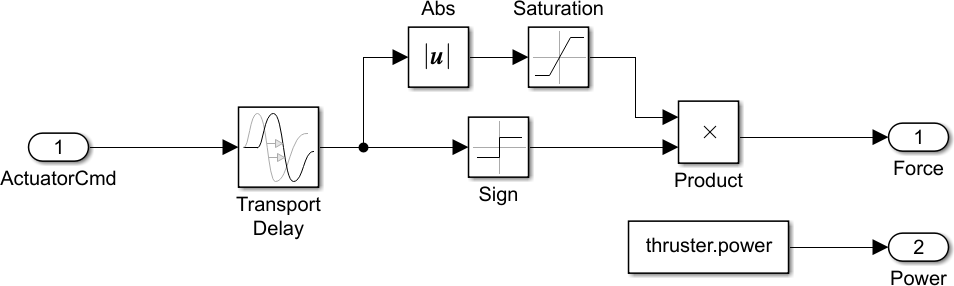
\includegraphics[width=1\textwidth]{2-toolbox/basic_thrusters.png}
            \caption{Directional Thruster model}
            \label{fig:basic_thrusters}
        \end{figure}

        One type of actuators that provide the source for external forces and torques acting on a spacecraft are gas thrusters. In case of small satellites, \ac{cgp} Systems are the most popular solution, since its simple design leads to smaller actuator mass and low power consumption. A \ac{cgp} system operates in a process of controlled ejection of compressed liquid or gas propellant. 
        
        Spacecraft thrusters can be applied for orbit change maneuvers, rapid attitude changes, momentum dumping, nutation and adjusting spin rates. The main advantage of gas propulsion is that the thrust can be controlled with high precision and they can provide high forces and torques. Moreover, there is no need for desaturation of a thrusters, in opposition to reaction wheels. Nevertheless the requirement for propellant posses a problem for small satellites, making it a rare method of attitude control in CubeSats and other micro- and nanosatellites. 
        
        The key parameters, available for set up in \ac{scars} Toolbox Thruster model are: thrust range, nominal thrust, specific impulse, amount of propellant, total impulse, power consumption, mass and time delay to control. Same as in Simple Actuators, noise sources can be set up.

        In \ac{scars} Parts Library various versions of Thruster are available:
        \begin{itemize}
            \item \textbf{Directional Thrusters} - Effective forces are assumed to be located on spacecraft body axes, leading to the lack of external torques, hence this model can be used for orbit corrections and maneuvers.
            \item \textbf{Rotational Thrusters} - Effective forces are assumed to be axisymmetric, therefore there are no forces generated by the thrusters, so this configuration can be used for pure attitude control. Additional parameter required for this model is radial displacement for the thrusters. 
            \item \textbf{Bang-Bang Thrusters} - Thrusters that operate in bang-bang control mode, allowing for operation only with no or maximum thrust. Additional parameters required for this model are turn-on and turn-off thresholds in control signal. They can be used either in orbit or attitude control and in respective cases they follow the principles of Directional and Rotational Thrusters.
        \end{itemize}

        \begin{figure}[H]
            \centering
            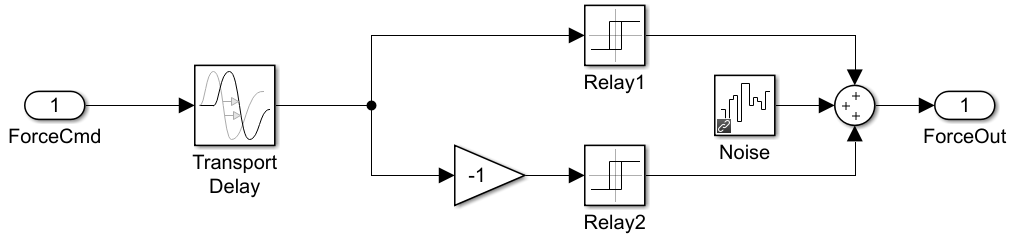
\includegraphics[width=1\textwidth]{2-toolbox/bang_bang.png}
            \caption{Bang-Bang Thruster model}
            \label{fig:bang_bang}
        \end{figure}


        For all thrusters models the only input is the control signal, while the outputs are fuel consumed and either generated force or torque. \ac{cgp} Systems also have a downside of decreasing thrust profile in relation with time, since thrust is correlated with the pressure of the propellant inside a tank. This property is not yet modeled in \ac{scars} Toolbox. %\dots\textit{should it be?}\dots

        % \begin{itemize}
        %     \item Thrust range;
        %     \item Nominal thrust \textit{(find a way to model change)}
        %     \item Specific impulse \textit{(and ranges)}
        %     \item Max propellant
        %     \item Total impulse
        %     \item Power consumption \textit{(at nominal thrust)}
        %     \item Mass
        %     \item Dimensions?
        %     \item Hot standby Power
        %     \item Time delay to control
        %     \item In both directions
        % \end{itemize}
        
        % \dots\textit{description of implementation}\dots

        % Bang-bang: https://apps.dtic.mil/dtic/tr/fulltext/u2/a291803.pdf
        % /resources/noise_description.pdf
        % \begin{figure}[H]
        %     \centering
        %     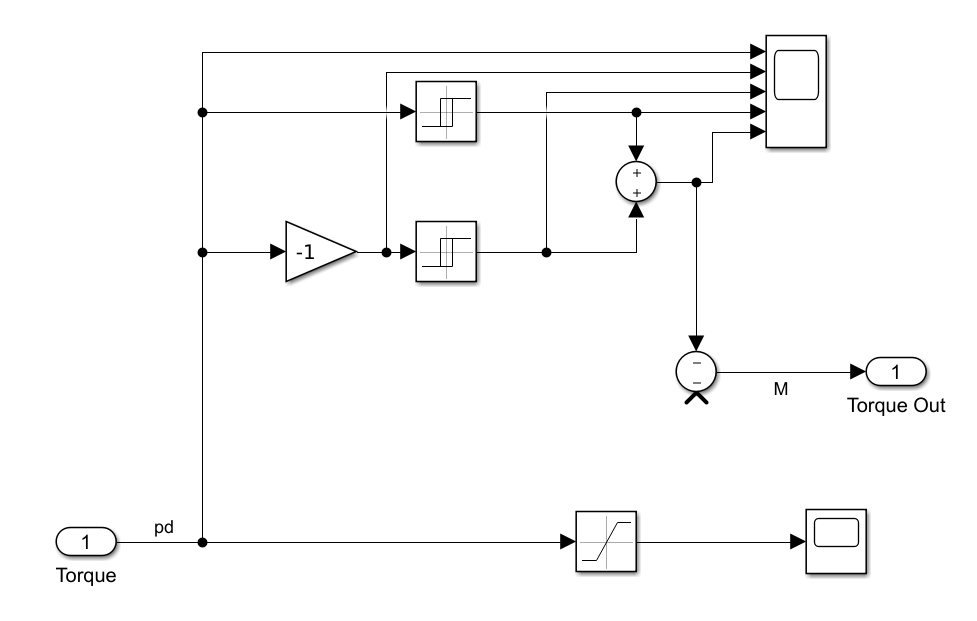
\includegraphics[width=1\textwidth]{2-toolbox/thru_simulink.png}
        %     \caption{Simulink Bang-Bang Thrusters model wrapper}
        %     \label{fig:bang_bang_simulink}
        % \end{figure}

    \subsubsection{Reaction Wheels}
        \begin{figure}[H]
            \centering
            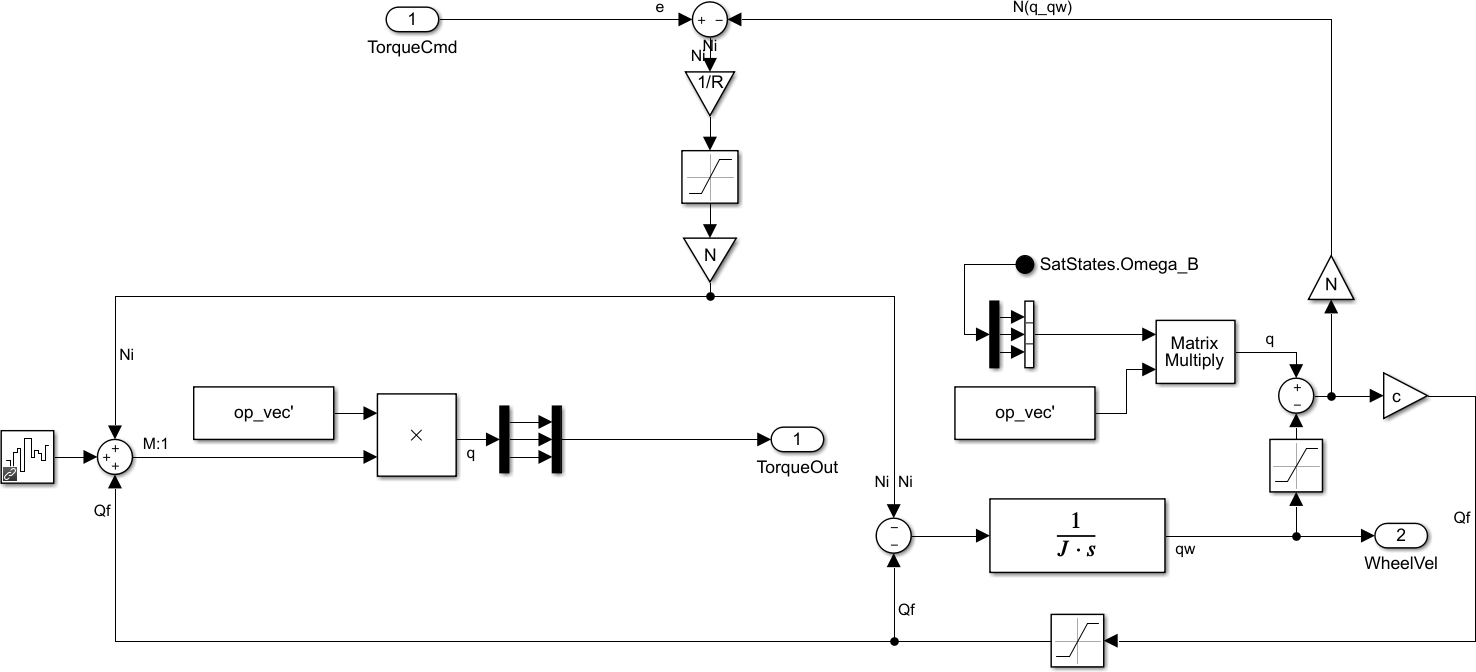
\includegraphics[width=1\textwidth]{2-toolbox/reaction_wheels.png}
            \caption{SCARS Reaction Wheel model}
            \label{fig:reaction_wheels}
        \end{figure}

        % Ideal to real: Bearing Noise, Transport Delay, Saturation, Quantization.
        
        Fast attitude control can be also achieved by the use of reaction wheels - mechanisms consisting of rotating flywheel and proportional electromagnetic torquer, such as DC motor. This allows very precise attitude maneuvers, with the possibility to eliminate most disturbance torques. Reaction wheels operate at around non-zero reference speed and change in their angular velocity imposes corresponding torque on the spacecraft. The disadvantage of this solution is that reaction wheels have fixed operating range and to achieve higher angular velocities for the spacecraft, the wheels have to be desaturated using another actuators. In CubeSats, for example, most commonly this would be solved by the addition of magnetorquers.

        In fast attitude control the motion around each spacecraft body axis can be considered to be decoupled from motion around two other axes. The equations of motion that describe the influence of reaction wheels angular velocity $\dot{q_w}$ on total angular momentum $H$ are as follows:
        
        % \begin{equation}
        \begin{align}
            I_y\dot{q} &= Ni+Q_f+Qdy\\
            \dot{\Theta} &= q\\
            J\dot{q_w} &= -Ni-Q_f\\
            Ri &= e - N(q-q_w)\\
            Q_f &= -c(q-q_w)\\
            H &= I_yq + Jq_w
        \end{align}
        % \end{equation}

        Where $e$, $i$, $R$ are respectively steering voltage, current in DC motor and armature resistance. $N$ is torque per unit current and $c$ is viscous friction coefficient. $Q_f$ is wheel bearing friction torque and $Q_{dy}$ stands for external disturbance torque. Said equations were modelled in the toolbox as it can be seen on \autoref{fig:reaction_wheels}. 

        The problem with modeling off-the-shelf reaction wheels is that datasheets rarely provide the value of viscous friction coefficient $c$ in the DC motor, therefore in \ac{scars} it is considered to be an optional parameter. 
        
        % Therefore to model this kind of actuator, \ac{scars} requires the user to only input following data, with $c$ being optional:
        
        % sources: bryson and this funny magnetorquer stuuff
        
        % \subsubsection{Gimbaled Momentum Wheel}

        %here goes the table


    \subsubsection{Magnetorquers}
        % sources - "magnetorquer and nice stuff" pdf and sidi maybe?

        \begin{figure}[H]
            \centering
            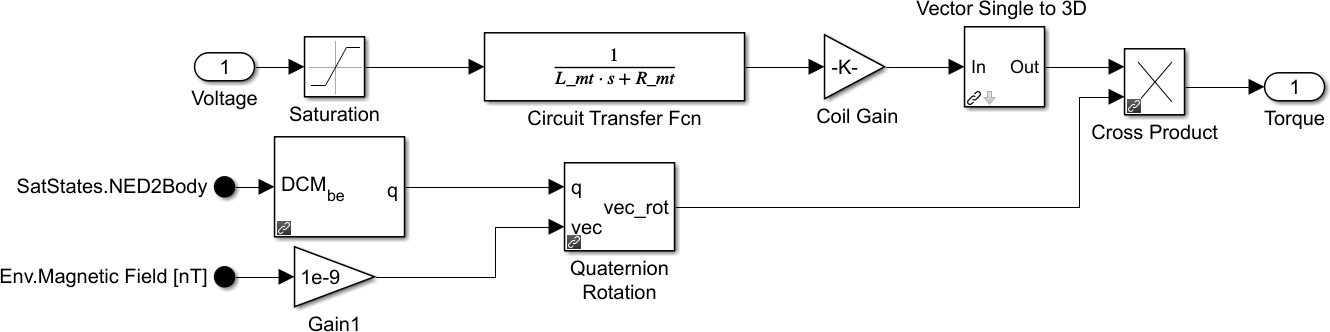
\includegraphics[width=1\textwidth]{2-toolbox/magnetorquer.png}
            \caption{SCARS Magnetorquer model}
            \label{fig:reaction_wheels}
        \end{figure}

        A magnetorquer is an attitude actuator which uses Earth's geomagnetic field to generate controlling torque. The active part in the magnetorquer is the solenoid, which generates the magnetic dipole moment proportional to the current conducted by the coil. This interaction is described with the following equation:

        \begin{align}
            \tau_B = M \times B
        \end{align}

        Where $\tau_B$ is mechanical torque acting on the spacecraft, $M$ the generated magnetic moment inside of it and $B$ is the magnetic field density. As the product of a skew-symmetric matrix and a vector it takes a form of:

        \begin{equation}
            \begin{bmatrix}
            \tau_{Bx}\\ 
            \tau_{By}\\ 
            \tau_{Bz}
            \end{bmatrix}
            \begin{bmatrix}
            0 & B_z & -B_y\\ 
            -B_z & 0 & B_x\\ 
            B_y & -B_x & 0
            \end{bmatrix}
            \begin{bmatrix}
            M_x\\
            M_y\\
            M_z
            \end{bmatrix}                
        \end{equation} % cite SIDI heres

        \ac{scars} Magnetorquer block models a torque rod, a solenoid with a magnetic core. The magnetic moment of a rod magnetorquer is a function of rod current and parameters of the coil, as described in following equation:

        \begin{equation}
            M = I_M\frac{\pi lw}{4d}\left[\left( \frac{\left[ \left( \frac{l}{w} \right) -1\right]^{3/2}}{\left( \frac{l}{w} \right)\cosh^{-1}\left( \frac{l}{w} \right)-\left[\left( \frac{l}{w} \right)^2 -1\right]^{1/2}} \right)- 1 \right]
        \end{equation}

        Where $l$ is the length of magnetic core, $w$ is the width of it and $d$ is the diameter of the wire. $I_M$ is the current flowing through the rod, which can be described with a transfer function, where $L$ is the solenoid's inductance and $R$ its resistance:

        \begin{equation}
            I_M = \frac{V_M}{Ls+R}
        \end{equation}

        % interesting problem with B matrix being singular, SIDI page 186 (204 in pdf)

        % cite: GOOD MAGNE CITE - 10.1.1.565.8909.pdf

        The drawback of using magnetorquers for attitude control is that they are unfit for fast maneuvers. Moreover, since Earth's magnetic field density is inversely proportional to cube of distance from Earth's center, then without high grade sensors or on-board models, they do not allow for precise maneuvering on higher orbits.


    \subsubsection{Drag Sail}
        \begin{figure}[H]
            \centering
            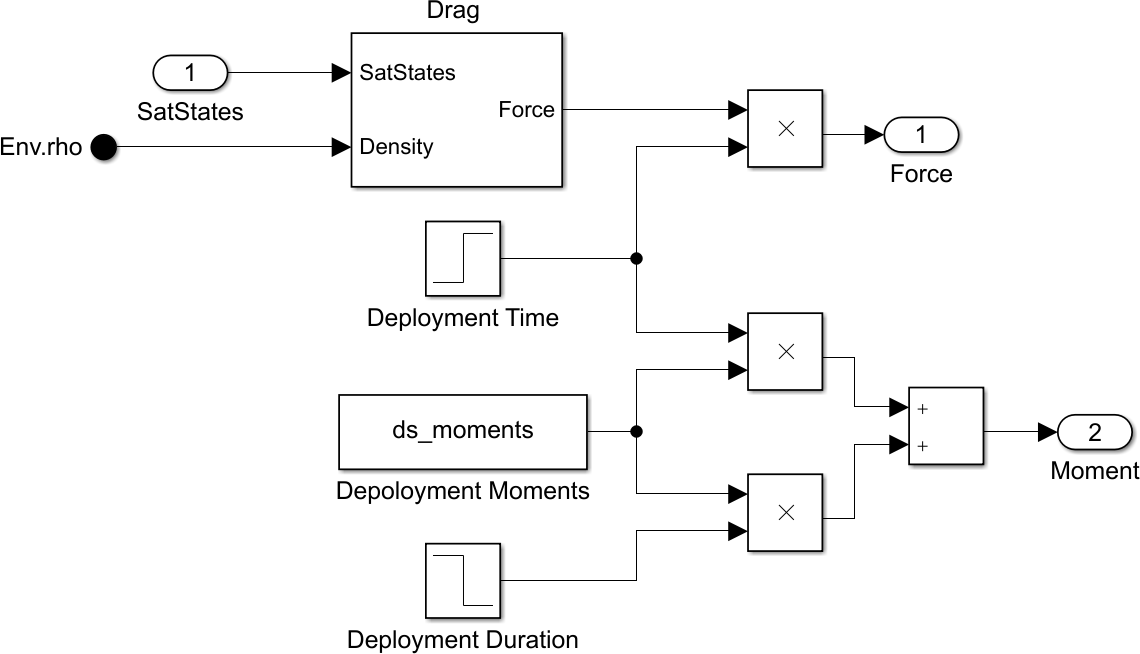
\includegraphics[width=1\textwidth]{2-toolbox/drag_sail.png}
            \caption{SCARS Drag Sail model}
            \label{fig:drag_sail}
        \end{figure}

        Drag sails use the occurrence of partial atmosphere (described in \ref{toolbox:atmosphere}) to lower satellite's tangential velocity and therefore to quicken the deorbitation of the spacecraft. The premise is to increase area-to-mass-ratio by deploying a large and lightweight structure near the planned end-of-life of the spacecraft. Due to this operating principle, drag sails are only relevant for low and medium mass spacecrafts and are applicable exclusively on \ac{leo}. To calculate the perturbing acceleration following equation is used:
        \begin{equation}
            F = -\frac{1}{2}\rho C_d A v^2sin\alpha
        \end{equation}
        Where $alpha$ is the angle between the sail's plane and satellite's velocity vector. Currently the moment of sail's deployment is not simulated in \ac{scars} toolbox.

